%---------------------------------------------------------------------------%
%-                                                                         -%
%-                           LaTeX Template                                -%
%-                                                                         -%
%---------------------------------------------------------------------------%
%- Copyright (C) Huangrui Mo <huangrui.mo@gmail.com> 
%- This is free software: you can redistribute it and/or modify it
%- under the terms of the GNU General Public License as published by
%- the Free Software Foundation, either version 3 of the License, or
%- (at your option) any later version.
%---------------------------------------------------------------------------%
%->> Document class declaration
%---------------------------------------------------------------------------%
% \documentclass[twoside]{Style/ucasthesis}%
\documentclass[oneside]{Style/ucasthesis}%
%- Multiple optional arguments:
%- [<oneside|twoside|print>]% oneside eprint, twoside eprint, or paper print
%- [fontset=<adobe|none|...>]% specify font set instead of automatic detection
%- [scheme=plain]% thesis writing of international students
%- [draftversion]% show draft version information
%- [standard options for ctex book class: draft|paper size|font size|...]%
%---------------------------------------------------------------------------%
%->> Document settings
%---------------------------------------------------------------------------%
\usepackage{caption}
\usepackage{pdfpages}
\usepackage[super,numbers, list,table,math]{Style/artratex}
%- usage: \usepackage[option1,option2,...,optionN]{artratex}
%- Multiple optional arguments:
%- [bibtex|biber]% set bibliography processor and package
%- [<numbers|super|authoryear|alpha>]% set citation and reference style
%- <numbers>: textual: Jones [1]; parenthetical: [1]
%- <super>: textual: Jones superscript [1]; parenthetical: superscript [1]
%- <authoryear>: textual: Jones (1995); parenthetical: (Jones, 1995)
%- <alpha>: textual: not available; parenthetical: [Jon95]
%- [geometry]% reconfigure page layout via geometry package
%- [lscape]% provide landscape layout environment
%- [xhf]% disable header and footer via fancyhdr package
%- [color]% provide color support via xcolor package
%- [background]% enable page background
%- [tikz]% provide complex diagrams via tikz package
%- [table]% provide complex tables via ctable package
%- [list]% provide enhanced list environments for algorithm and coding
%- [math]% enable some extra math packages
%- [xlink]% disable link colors
\usepackage{Style/artracom}% user defined commands
%---------------------------------------------------------------------------%
%->> Document inclusion
%---------------------------------------------------------------------------%
%\includeonly{Tex/Chap_1,...,Tex/Chap_N}% selected files compilation
%---------------------------------------------------------------------------%
%->> Document content
%---------------------------------------------------------------------------%
%-
%-> Titlepage information
%-
%---------------------------------------------------------------------------%
%->> Titlepage information
%---------------------------------------------------------------------------%
%-
%-> 中文封面信息
%-
\schoollogo{scale=0.112}{ucas_logo}% 校徽
\title{xxxx}% 题目
\author{张三}%作者姓名
\authorid{202xxx}% 学号
\advisor{xxx}% 指导老师
\advisortitle{xxx}% 指导老师职务
\degree{学位}% 学位:硕士、博士,按照填表说明填写
\degreetype{按照填表说明填写}% 学位类别,按照填表说明填写
\major{按照填表说明填写}% 二级学科专业名称
\field{研究方向}% 研究方向
\institute{院所}% 院所
%---------------------------------------------------------------------------%
%

\begin{document}
%-
%-> Frontmatter: title page, abstract, content list, symbol list, preface
%-
\frontmatter% initialize the environment

%---------------------------------------------------------------------------%
%->> Frontmatter
%---------------------------------------------------------------------------%
%-
%-> 生成封面
%-

\maketitle% 生成中文封面
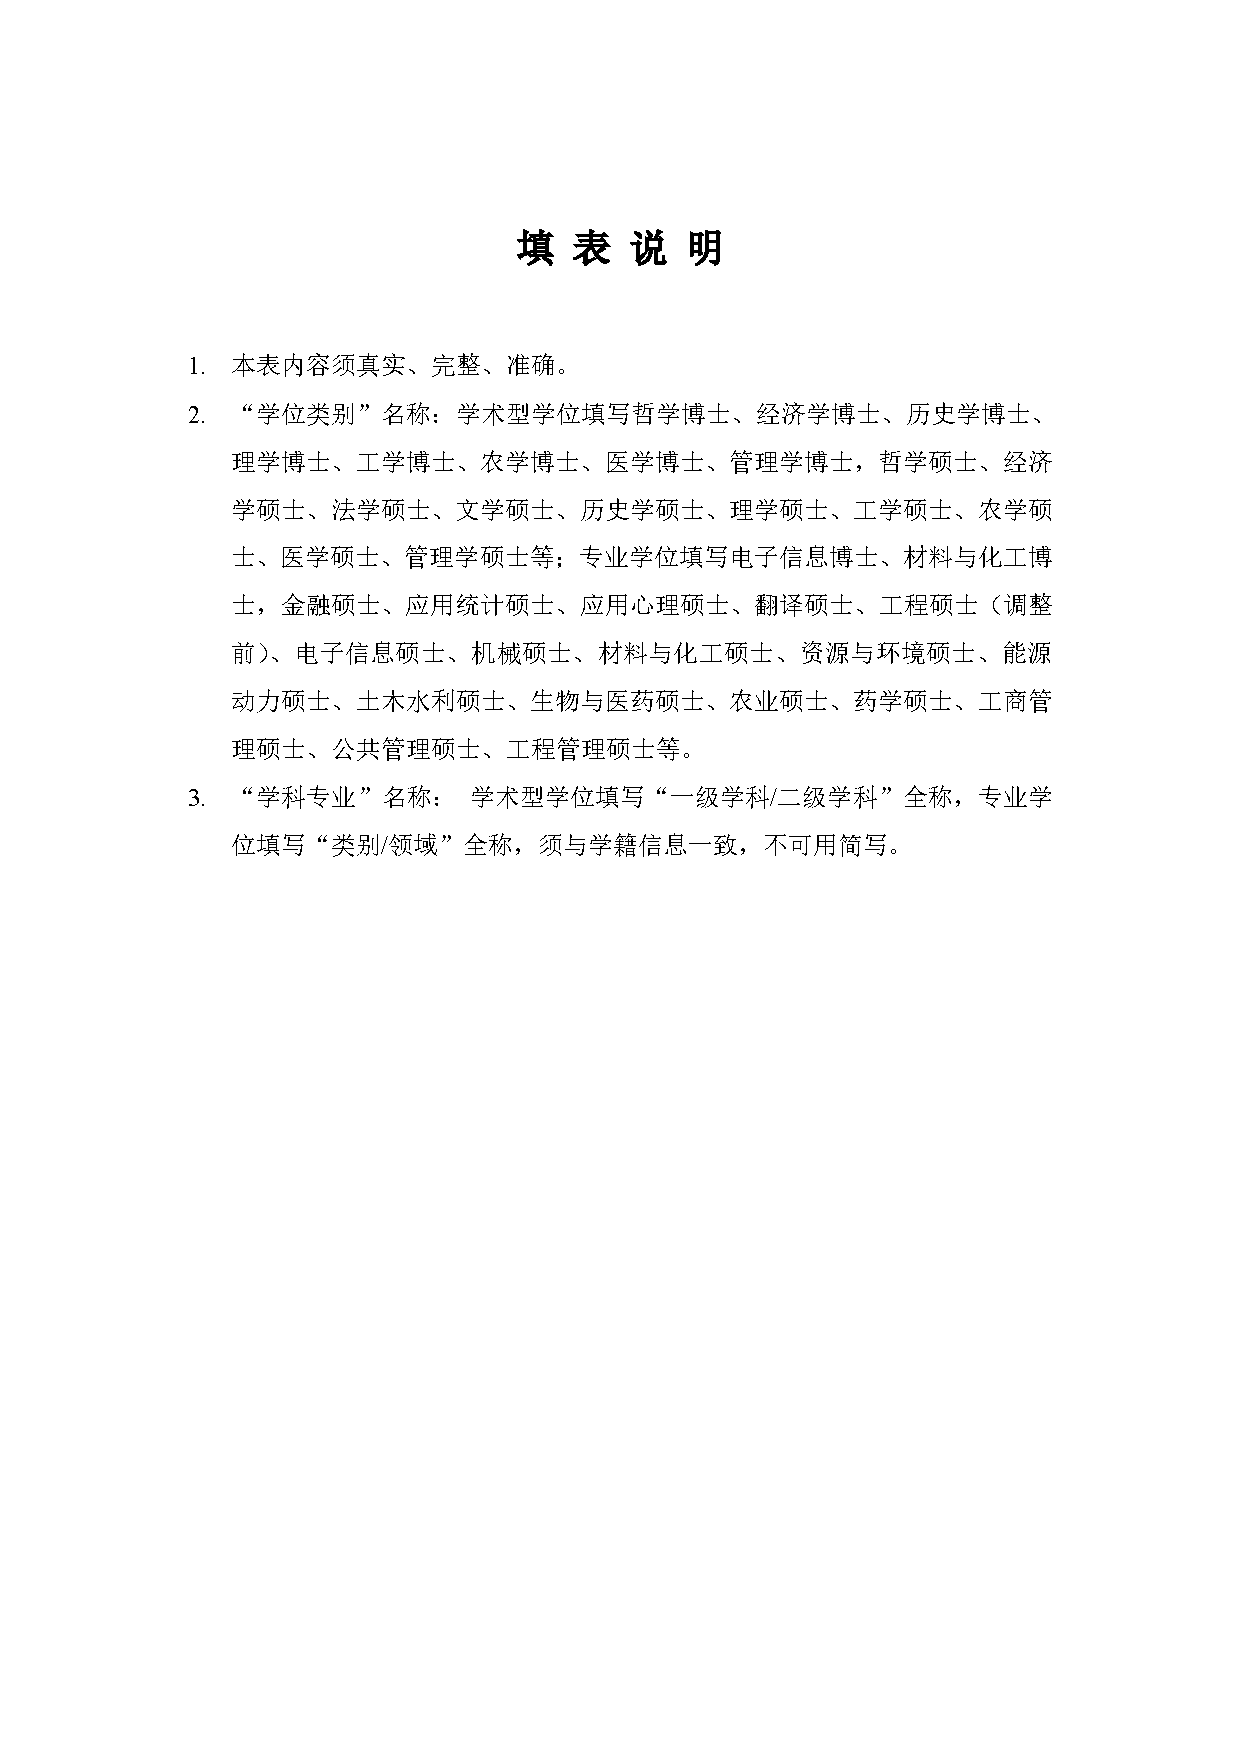
\includepdf[pages=1-2]{Tex/Interim.pdf}
% \MAKETITLE% 生成英文封面
% %-
% %-> 作者声明
% %-
% \makedeclaration% 生成声明页
% %-
% %-> 中文摘要
% %-
% \intobmk\chapter*{摘\quad 要}% 显示在书签但不显示在目录
\setcounter{page}{1}% 开始页码
\pagenumbering{Roman}% 页码符号

% 中文摘要、英文摘要、目录、论文正文、参考文献、附录、致谢、攻读学位期间发表的学术论文与其他相关学术成果等均须由另页右页(奇数页)开始。

% \keywords{中国科学院大学,学位论文,模板}% 中文关键词
% %-
% %-> 英文摘要
% %-
% \pagestyle{frontmatterstyle}%
% \intobmk\chapter*{Abstract}% 显示在书签但不显示在目录
% \pagestyle{enfrontmatterstyle}%

% Chinese abstracts, English abstracts, table of contents, the main contents, references, appendix, acknowledgments, author's resume and academic papers published during the degree study and other relevant academic achievements must start with another right page (odd-numbered page).

%     %- the current style, comment all the lines in plain style definition.

% \KEYWORDS{University of Chinese Academy of Sciences, Thesis, LaTeX Template}% 英文关键词

% \cleardoublepage\pagestyle{frontmatterstyle}%
% \cleardoublepage
\clearpage

%---------------------------------------------------------------------------%
% title page, abstract
{% content list region
\linespread{1.2}% local line space
\intobmk*{\cleardoublepage}{\contentsname}% add link to bookmark
% \newpage

\tableofcontents% content catalog
\intobmk*{\cleardoublepage}{图表目录}
\pagestyle{figureheader}
\input{Tex/figuretable}

}
\thispagestyle{figureheader}
\input{Tex/Prematter}% symbol list, preface content
%-
%-> Mainmatter
%-
\mainmatter% initialize the environment

\input{Tex/Mainmatter}% main content
%-
%-> Appendix
%-

%-
%-> Backmatter: bibliography, glossary, index
%-

\intotoc*{\cleardoublepage}{\bibname}% add link to toc
\artxifstreq{\artxbib}{bibtex}{% enable bibtex
    \bibliography{Biblio/ref}% bibliography
}{%
    \printbibliography% bibliography
}
\cleardoublepage%
% \appendix% initialize the environment
% \input{Tex/Appendix}% appendix content

% \thispagestyle{appendixheader}
% \backmatter% initialize the environment
% \input{Tex/Backmatter}% other information
\end{document}
%---------------------------------------------------------------------------%

